\chapter{基于深度学习的目标检测技术}
\label{chap:2}

\section{目标检测研究进展}
目标检测是计算机视觉领域重要的研究方向,有着长达20年的研究进程。目标检测任务通常被描述为:给定一张图像或者视频桢,定位其中所有感兴趣的目标,并确定每个目标的具体类别。图像中的目标可能出现在任何位置,目标的尺度和形态也存在各种各样的变化,图像的背景更是千差万别,这些因素导致目标检测并不是一个容易解决的问题。

目标检测第一个比较成功的案例,就是在大概2000年前后出现的Viola-Jones人脸检测器 \cite{viola-jones} \cite{via-jones-face}。这个方法的基本思路就是滑动窗口式的,用一个固定大小的窗口在输入图像上滑动,将窗口选定的图像区域送入分类器判断是人脸还是非人脸。滑动窗口的大小是固定,但是人脸的大小则各种各样,为了检测不同大小的人脸,还需要将输入图像缩放到不同大小,使得各种大小的人脸都能够在某个尺度上与窗口大小匹配。这种滑动窗口式的方法存在一个明显的问题,就是有太多的候选窗口去判断是人脸还是非人脸。为了加速这一过程,Viola-Jones检测器采用了级联的AdaBoost分类器,这种级联的结构能够逐级地过滤掉大量的非人脸窗口。值得一提的是,Viola-Jones人脸检测器之后被广泛应用在大量的电子产品中,例如数码相机中的人脸对焦功能,照相的时候,相机会自动检测人脸,然后根据人脸的位置把焦距调整得更好。

2005年出现的HOG特征描述子 \cite{hog} 是目标检测领域另一个里程碑式的进步。HOG是Histograms of Oriented Gradients的缩写,最早被应用在行人检测任务中。它的基本思想就是通过梯度或边缘的方向密度分布来表征一个对象,这种特征对于轮廓明显的对象具有较好的描述能力。HOG特征结合SVM分类器在行人检测领域大获成功,之后虽然有很多行人检测算法不断提出,但大多都是以HOG+SVM为基本框架。HOG特征对图像的几何和光学变化都能保持很好的不变性,不仅可以用来检测行人,也可以用来检测猫、狗等几乎任何物体。HOG的出现使得Viola-Jones检测器不再是目标检测的唯一选择。

继Viola-Jones检测器和HOG特征描述子之后,在2009年了出现了另外一个比较重要的方法:可变形部件模型 (Deformable Part Model,DPM)\cite{dpm}。目标大体上可以分为两类,刚性物体和非刚性物体。刚性物体,例如人脸,通常情况下不会有非常大的形变,比如嘴巴变到鼻子的上面,这类目标通常比较容易解决。非刚性物体,例如人体,可以看作一系列非刚性部件的铰接组合。DPM通过对部件进行建模可以很好地处理这种非刚性物体,它同时基于局部的部件和整体去做分类,在行人和车等任务上取得了较大的突破。DPM引入了对部件的建模,本身是一个很好的方法,但是被深度学习的光芒给盖过去了。深度学习对目标检测的精度带来了巨大的提升,所以研究DPM的一些学者也快速转移到深度学习上去了。

\begin{figure}[!t]
	\centering
	\includegraphics[scale=0.7]{detection_flow}
	\caption{传统目标检测算法的一般流程。}
	\label{detection_flow}
\end{figure}

总结下来,如图 \ref{detection_flow} 所示,传统的目标检测方法一般分为三个阶段:首先在给定图像上选择一些候选区域,然后对这些候选区域对应的图像块提取特征,最后使用预先训练好的分类器进行分类。
\begin{namelist}{}
	\item (1) 候选区域选择。\\
	由于目标可能出现在图像的任何位置,而且目标的尺度和长宽比也不确定,所以传统方法大多采用滑动窗口的机制对整幅图像进行遍历,而且需要设置不同的窗口大小和长宽比进行多次遍历。这种穷举的策略虽然包含了目标可能出现的所有位置,但是时间复杂度太高,而且冗余窗口太多容易增加``虚警率''。
	\item (2)特征提取。\\
	特征提取的好坏直接影响到分类的准确性,设计一个鲁棒的特征是研究人员坚持不懈的追求。然而,由于目标形态的多样性,图像背景的差异性等因素,研究人员手工设计的特征大多适用于特定目标种类,例如Haar \cite{via-jones-face},LBP \cite{lbp} 特征适用于人脸检测,HOG特征则对行人检测表现良好。
	\item (3)候选区域分类。\\
	分类器将候选区域判别为背景或者某个具体类别。目标检测任务中常用的分类器有SVM,AdaBoost等。
\end{namelist}
传统目标检测算法主要存在两个问题:一个是基于滑动窗口的机制没有针对性,时间复杂度高,窗口冗余;二是手工设计的特征对于目标和背景的多样性变化不具备很好的鲁棒性。

\section{基于Region Proposal的深度学习目标检测算法}
对于传统目标检测算法中存在的两个问题,基于Region Proposal的深度学习目标算法给出了解决方案。

针对滑动窗口存在的问题,region proposal提供了解决办法。Region proposal(候选区域)就是图像中可能存在目标的位置。利用纹理、边缘、颜色等底层图像信息,region proposal提取算法能够保证在选取较少窗口(几千个甚至几百个)的情况下保持较高的目标召回率。这大大降低了后续计算的复杂度,并且获取的候选窗口甚至比滑动窗口的质量更高(滑动窗口通常以一定歩幅滑动)。比较常用的region proposal提取算法有selective search \cite{selective-search},edge box \cite{edge-box}和MCG \cite{mcg}。

有了候选区域,剩下的工作就是对候选区域对应的图像块进行分类。对于图像分类任务,深度卷积神经网络(Deep Convolutional Neural Network, DCNN)取得了巨大的突破。在2012年的ImageNet大规模视觉识别挑战赛(ILSVRC)上,Krizhevsky使用深度卷积神经网络AlexNet \cite{alexnet}将图片分类任务的top5-error降低到了15.3\%,而使用传统方法的第二名top5-error高达26.2\%。最新的神经网络,如ResNet \cite{resnet},Inception V4 \cite{inception-v4}等,已经将top5-error降到了4\%以内。2014年Ross B. Girshick等使用region proposal和DCNN代替传统方法使用的滑动窗口和手工设计特征,设计了R-CNN \cite{rcnn}目标检测框架,将PASCAL VOC 2010 \cite{pascal-voc-2010} 目标检测任务的state of the art由35.1\%提升到53.7\%,使得目标检测取得了巨大突破。

本节首先简要介绍一下深度卷积神经网络,然后介绍R-CNN目标检测框架及其加速改进版本SPP-net,Fast R-CNN,Faster R-CNN,并分析现有算法的不足,然后在下一节介绍本文提出的目标检测算法。

\subsection{深度卷积神经网络}
如图 \ref{cnn} 所示,一个简单的卷积神经网络由各种不同的层按照顺序排列组成。卷积神经网络主要由四种类型的层构成:卷积层(CONV),RELU层,池化层(POOL)和全连接层(FC),其中全连接层和常规神经网络中的一样。通过将这些层叠加起来,就可以构成一个完整的卷积神经网络。图 \ref{cnn} 中网络在CIFAR-10图像分类任务中的前向计算过程如下:
\begin{namelist}{}
	\item (1)输入有RGB三个颜色通道的图像构成输入层,CIFAR-10中图像宽高均为32,即输入数据体的维度为$32\times32\times3$。
	\item (2)卷积层中每个神经元与输入层中的一个局部区域相连接,每个神经元计算与自己相连接的小区域与自己权重的内积。卷积层会计算所有神经元的输出,如果我们使用12个滤波器(也称作卷积核),得到的输出数据体的维度就是$32\times32\times12$。
	\item (3) RELU层进行element-wise的激活函数操作,使用以零为阈值的$\max(0,x)$作为激活函数。该层对数据维度没有改变,输出数据体的维度还是$32\times32\times12$。
	\item
	(4)池化层在空间维度(宽度和高度)上进行降采样(downsampling)操作,输出数据体的维度变为$16\times16\times12$。
	\item
	(5)全连接层计算各个类别的评分,数据维度变为$1\times1\times10$,10路输出分别对应CIFAR-10中10个类别的评分值。全连接层与常规神经网络一样,每个神经元都与前一层中所有神经元相连接。
\end{namelist}
\begin{figure}[!t]
	\centering
	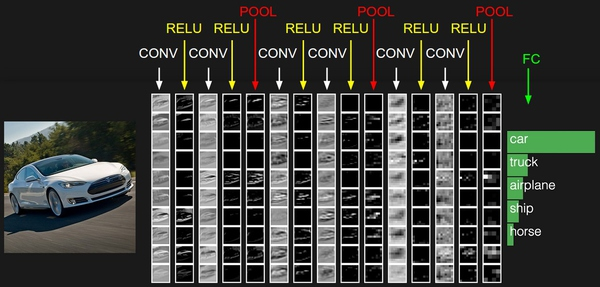
\includegraphics[width=\textwidth]{cnn}
	\caption{深度卷积神经网络在CIFAR-10 \cite{cifar-10} 图像分类任务上的应用示意图。注意:图中池化层的输出与输入具有相同的尺寸,这仅仅是为了示意,实际运行中池化层会进行降采样。输出层只显示了5个得分最高的评分值和对应的类别。}
	\label{cnn}
\end{figure}

\subsubsection{卷积层}
卷积层是卷积神经网络的核心层。卷积层的参数由一组可学习的滤波器组成。每个滤波器在空间上(宽度和高度)都比较小,但是深度和输入数据一致,例如AlexNet \cite{alexnet} 网络第一个卷积层的滤波器尺寸为$11\times11\times3$(宽高都是11像素,输入图像有3个颜色通道,所以深度为3)。前向计算的时候,每个滤波器在输入数据体的宽度和高度上滑动,并计算滤波器在每个位置处的响应,生成一张2-D的激活图。经过训练,网络会让滤波器学习到当它探测到某些类型的视觉特征时就激活,例如某些方向上的边缘,甚至可以是网络更深层上的蜂巢状或车轮状图案。卷积层上每个滤波器都会生成一张不同的2-D激活图,将这些激活图在深度方向上层叠起来就生成了卷积层的输出数据体。滤波器的数目就是卷积层在深度方向上的神经元数目。

\begin{figure}[!t]
	\centering
	\includegraphics[width=\textwidth]{conv}
	\caption{\textbf{左边:}红色的部分表示输入数据体(例如CIFAR-10中的图像),蓝色的部分表示卷积层中的神经元。卷积层中的神经元与输入数据体在空间上局部相连,在深度维度上全部相连(所有颜色通道)。同一深度上的所有神经元共享一个滤波器,沿深度方向上的多个神经元(本例中5个)接受输入数据的同一块区域(感受野相同)。\textbf{右边:}与传统神经网络类似,单个神经元计算输入与权重的内积,然后进行激活函数运算;与传统神经网络不同的是,卷积层神经元的输入被限制在一个局部空间。}
	\label{conv}
\end{figure}

如图 \ref*{conv} 所示,卷积层与传统神经网络的区别在于神经元的连接方式,以及连接的参数共享模式:
\begin{namelist}{}
	\item (1)局部连接。\\
	在处理图像这样的高维度输入时,让每个神经元与前一层中的所有神经元相连是不现实的。因此卷积神经元只与输入数据的一个局部区域连接。该连接的空间大小叫做神经元的感受野(receptive field),它的尺寸就是滤波器的空间尺寸。在深度方向上,这个连接是全连接,和深度方向上的所有神经元相连,如图 \ref{conv} 所示。
	\item (2)参数共享。\\
	卷积层同一深度上的所有神经元共享一个滤波器,这种机制称作参数共享。卷积层使用参数共享来控制参数的数量,减小过拟合的风险。除此以外,参数共享机制还满足``平移不变性'':如果一个特征在位置$(x_1,y_1)$处被激活,那么将它平移至$(x_2,y_2)$处也应该被激活,这一特性对于图像分类大有益处 \cite{mnist}。如果将深度维度上一个单独的2-D切片看作深度切片,则在一个深度切片上的所有神经元使用同一个权重向量,那么卷积层的前向计算在每个深度切片中可以看作是神经元权重与输入数据体的卷积(这就是``卷积层''名字的由来)。这也是为什么这些权重集合称为滤波器(filter)(或卷积核(kernel))。
\end{namelist}

\subsubsection{RELU层}
首先声明,ReLU层其实是一个激活函数,对应图 \ref{conv} 中右半部分的$f$。下文中所称ReLU神经元也是指使用ReLU激活函数的神经元。传统神经网络中最常用的两个激活函数,Sigmod系(Logistic-Sigmoid和Tanh-Sigmod)对中央区的信号增益较大,对两侧区的信号增益小。从神经科学上看,中央区酷似神经元的兴奋态,两侧区酷似神经元的抑制态,因而在神经网络学习方面,可以将重点特征推向中央区,非重点特征推向两侧区。Sigmod系激活函数推动了早期神经网络的发展。另一方面,Sigmod系激活函数也容易导致一个臭名昭著的问题,梯度消失问题(Gradient Vanishing Problem)。误差从输出层反向传播计算梯度时,在各层都要乘当前层的输入神经元值和激活函数的一阶导数,即
\begin{equation}
\frac{\partial l}{\partial \omega_c}=\frac{\partial l}{\partial x_{c+1}}\cdot f'\cdot x_c
\end{equation}
其中$l$表示损失函数,$c$表示当前层,$\omega_c$表示当前层的权重,$x_c$表示当前层的输入神经元值,$f$表示激活函数。具有双端饱和特性的Sigmod系激活函数会有以下两个问题:
\begin{namelist}{}
	\item (1)$f'\in (0, 1)$,而且饱和区内接近于0,导致导数缩放;	
	\item (2)激活值$x\in (0,1)$或$x\in (-1,1)$,导致饱和值缩放。
\end{namelist}
这样每经过一层,梯度值都是成倍的衰减,一旦进行递推式的多层反向传播,梯度就会不停的衰减,消失,使得网络学习变慢。由于梯度消失问题的存在,使得长期以来深度神经网络的训练都十分困难,也导致了神经网络研究的停滞。

近些年ReLU(Rectified Linear Unit)\cite{relu} 激活函数变得非常流行,它的函数公式是$\max(0,x)$。如图 \ref{fig:relu} 所示,这个激活函数是一个单侧响应的线性单元。相较于Sigmod系激活函数,ReLU对于随机梯度下降的收敛有巨大的加速作用,AlexNet \cite{alexnet} 论文里指出有6倍之多。这主要归功于它的线性和非饱和性。Sigmod系函数含有指数运算等耗费计算资源的操作,而ReLU可以简单地通过对一个数组进行阈值操作即可。但是在训练的时候,ReLU单元比较脆弱并且可能``死掉''。例如,当一个很大的梯度流过ReLU的神经元后,可能会导致神经元更新到一种特别的状态,在这种状态下神经元将无法被其他任何输入再次激活。如果这种情况发生,那么从此流过该神经元的梯度都将变成0。也就是说,这个ReLU单元在训练中将不可逆转地死亡,这样会导致数据多样性的丢失。通过合理设置学习率,可以降低ReLU神经元死亡的概率。

\begin{figure}[h]
	\centering
	\includegraphics[scale=1]{relu}
	\caption{ReLU激活函数}
	\label{fig:relu}
\end{figure}

\subsubsection{池化层}
通常在连续的卷积层之后会周期性地插入一个池化层。它的作用是逐渐降低数据体的的空间尺寸,这样就可以减少网络中参数的数量,使得计算资源消耗变少,还能有效地抑制过拟合。池化层经常使用MAX操作,在某一个空间区域中取最大值(常见的区域大小为$2\times2$)。池化层对输入数据体的每一个深度切片独立进行操作,改变它的空间尺寸。除了MAX池化,池化单元还可以使用其他的函数,比如\emph{平均池化}(average pooling)或\emph{L2范式池化}(L2-norm pooling)。平均池化历史上比较常用,但是现在已经很少用了,因为实践证明,MAX池化的效果往往比平均池化的效果要好。虽然如此,平均池化操作依然有其用武之地,例如在最近的ParseNet \cite{parsenet} 中,平均池化被用于汇聚全图的上下文信息。

卷积神经网络最常见的形式就是将一些卷积层和RELU层放在一起,其后紧跟池化层,然后重复如此直到数据体在空间上被缩小到一个足够小的尺寸,在某个地方过渡成全连接层。最后的全连接层得到输出,比如分类评分。这种结构形式的卷积神经网络比较有名的几种为:LeNet \cite{mnist},AlexNet \cite{alexnet},ZF Net \cite{zfnet}, VGGNet \cite{vgg} 等。在卷积神经网络的相关文献中,中间层输出的激活图也被称为\emph{特征图}(feature map),下文会不加区分地使用这两个术语。

\subsection{R-CNN目标检测框架}
如本节引言中所介绍的,R-CNN目标检测框架借助region proposal方法和深度卷积神经网络来克服传统目标检测算法中的两个难点,显著提升了目标检测的精度。2014年的时候Ross B. Girshick等首次提出R-CNN检测算法,检测流程如图 \ref{fig:rcnn} 所示,可以分为4个阶段:
\begin{namelist}{}
	\item (1)输入测试图像。
	\item (2)采用selective search算法在图像中提取2000个左右的region proposal。
	\item (3)将每个region proposal缩放(warp)成$227\times227$的大小并输入到卷积神经网络(CNN),使用CNN全连接层的输出作为特征。
	\item (4)将每个region proposal提取到的CNN特征输入到SVM进行分类。
\end{namelist}

\begin{figure}[h]
	\centering
	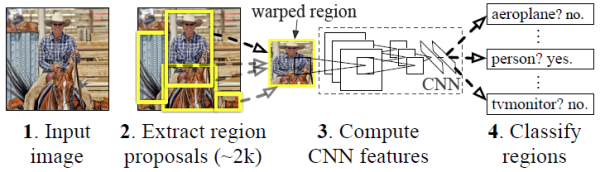
\includegraphics[width=\textwidth]{rcnn}
	\caption{R-CNN目标检测流程。R-CNN首次被提出的时候,卷积神经网络选用的是AlexNet。}
	\label{fig:rcnn}
\end{figure}

图 \ref{fig:rcnn} 所示的是R-CNN的测试流程图,要进行测试我们首先要训练好提取特征的CNN模型,以及用于分类的SVM:使用在ImageNet上预训练的AlexNet模型进行微调(fine-tune)得到用于特征提取的CNN模型,然后利用CNN模型对训练集提取特征训练SVM。训练和测试都需要将每个region propsoal缩放到同一尺度,因为CNN的全连接层需要固定维度的输入。而且图 \ref{fig:rcnn} 中省略了一个过程:对SVM分好类的region proposal进行边框回归(bounding box regression)。边框回归是对region proposal进行位置纠正的线性回归算法,为了让region proposal提取到的窗口跟目标真实窗口更加吻合。因为region proposal提取到的窗口不可能跟人手工标记的那么准,如果region proposal跟目标位置偏移较大,即便是分类正确了,但是由于region propsoal跟ground-truth窗口的IoU(Intersection over Union)低于0.5,那么目标相当于还是没有检测到。

R-CNN将PASCAL VOC 2010 \cite{pascal-voc-2010} 目标检测任务的state of the art由35.1\%提升到53.7\%,如此大的性能提升使研究目标检测的学者们看到了region proprosal+CNN这种框架的巨大优势。但是R-CNN也存在着很多问题,比如:
\begin{namelist}{}
	\item (1)训练分为多个阶段,步骤繁琐:微调网络+训练SVM+训练边框回归器。
	\item (2)训练耗时,磁盘开销大:5000张图片产生几百个GB的特征文件。
	\item (3)速度慢:对这2000个左右的region proposal都要执行一遍CNN的前向计算,运行在现代的GPU上依然需要47s来检测一张图片。
\end{namelist}

\subsubsection{SPP-net}
为了实现对R-CNN的加速,何凯明等随后提出了SPP-net \cite{sppnet},其做法是对整幅图像执行一次CNN前向计算,然后只需要将region proposal在原图的位置映射到卷积层特征图上,这样对于一张图像我们只需要提取一次卷积层特征,最后将每个region proposal的卷积层特征输入到全连接层做后续操作。但是这样有一个小困难,就是这2000个region proposal每一个的大小都不一样,直接这样输入全连接层肯定是行不通的,因为全连接层需要固定维度的输入。为了解决这个问题,SPP-net设计了空间金字塔采样(Spatial Pyramid Pooling,SPP),使得不同大的小窗口具有相同维度的特征,如图 \ref{fig:sppnet} 所示。

将一张任意尺寸的图像输入到CNN,经过卷积操作得到卷积特征(比如VGG16最后的卷积层为\texttt{conv5\_3},共产生512张特征图)。图 \ref{fig:sppnet} 中的 ``window''就是原图一个region proposal对应到特征图的区域,只需要将这些不同大小``window''的特征映射到相同的维度,就可以将其作为全连接层的输入。SPP-net中空间金字塔采样的具体做法为:将每个``window''划分为$4\times4$,$2\times2$,$1\times1$的空间网格,然后在每个网格内使用MAX池化进行降采样,这样对于每个``window''经过SPP层之后都得到了一个维度为$(4\times4+2\times2+1\times1)\times512$的特征向量,并将它作为全连接层输入进行后续操作。

SPP-net数十倍地提升了R-CNN的目标检测速度,但是也存在一些问题:
\begin{namelist}{}
	\item (1)训练分为多个阶段,步骤繁琐: 微调网络+训练SVM+训练训练边框回归器。
	\item (2) SPP-net在微调网络的时候固定了卷积层,只对全连接层进行微调,而对于目标检测任务,有必要对卷积层也进行微调,分类的模型提取的特征更注重高层语义,而目标检测任务除了语义信息还需要目标的位置信息。
\end{namelist}

\begin{figure}[!t]
	\centering
	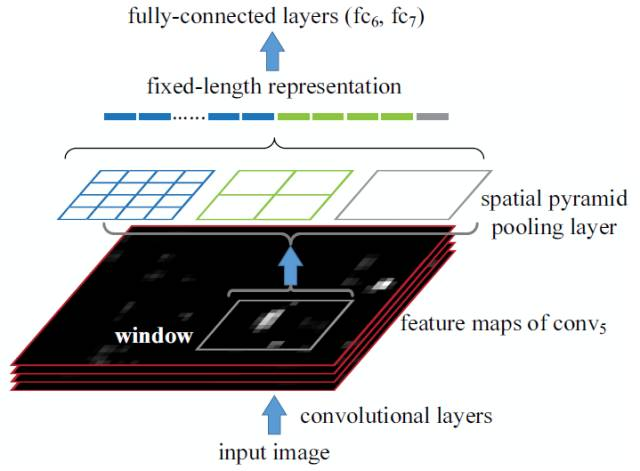
\includegraphics[width=0.8\textwidth]{sppnet}
	\caption{SPP-net中的spatial pyramid pooling做法示意图。}
	\label{fig:sppnet}
\end{figure}

\subsubsection{Fast R-CNN}
Fast R-CNN \cite{fast-rcnn} 借鉴了SPP-net的做法,在整幅图像上进行卷积,然后采用ROI-pooling对所有region proposal都得到固定维度的特征向量,并且实现了end-to-end的训练,大大提高了训练效率,而且能够对所有的层进行微调(在实际训练中将底层卷积层的参数固定防止过拟合)。Fast R-CNN的框架图如图 \ref{fig:fast-rcnn} 所示。
\begin{figure}[t]
	\centering
	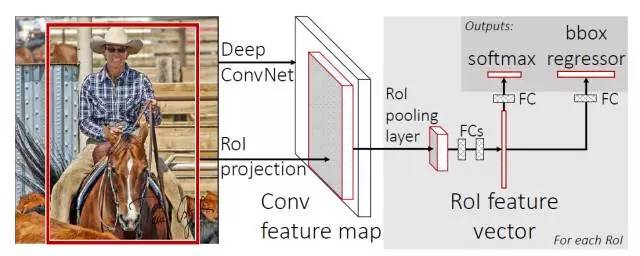
\includegraphics[scale=0.6]{fast-rcnn}
	\caption{Fast R-CNN检测算法框架图。}
	\label{fig:fast-rcnn}
\end{figure}

与SPP-net框架对比,Fast R-CNN主要有两处不同:
\begin{namelist}{}
	\item (1)最后一个卷积层后加了一个ROI-pooling层而不是SPP层。ROI-poolng层其实是SPP层的一个精简版,SPP层对每个region proposal使用了不同大小的网格进行降采样,而ROI-pooling只采用了一个$7\times7$大小的网格进行降采样。VGG16的最后一个卷积层\texttt{conv5\_3}有512张特征图,这样所有region proposal的特征向量维度都是$7\times7\times512$。 
	\item (2)SPP-net的训练过程分为三个阶段,而Fast R-CNN直接使用softmax替代SVM分类,并且梯度可以穿过ROI-pooling层到达卷积层,同时利用多任务损失函数同时学习类别和边框回归,这样整个训练过程就是端到端(end-to-end)的(除去region proposal提取阶段)。
\end{namelist}
Fast R-CNN将分类和边界框回归放到一起来做,才用了多任务协同学习的方式,不仅提升了训练和测试的效率,也小幅度地提升了目标检测的精度。

\subsubsection{Faster R-CNN}
使用Fast R-CNN进行目标检测,时间大多消耗在object proposal的提取上了,selective search \cite{selective-search} 算法对一张典型尺寸的图片提取region proposal需要2\textasciitilde 3s,而特征提取、分类和回归一共需要0.3s左右。而且在region proposal + CNN分类这种目标检测框架中,region proposal质量的好坏直接影响到目标检测任务的精度。如果找到一种方法只提取几百个或者更少的高质量的预选窗口,而且召回率很高,这不但能加快目标检测速度,还能提高目标检测的性能(假阳例少)。于是Faster R-CNN \cite{faster rcnn} 算法应运而生。

Faster R-CNN相比于Fast R-CNN将产生region proposal这一步也用深度网络来做,并且让这个网络和Fast R-CNN的分类网络共享卷积层,这个产生region propsal的网络叫做RPN(Region Proposal Networks),是Faster R-CNN的核心。RPN替代了之前非常慢的selective search,而且通常所用的region proposal的数目也比较少,只需要300个就够了,这使得后面分类的速度会更快。为了检测各种各样的物体,RPN引入了所谓anchor box的设计,具体来说,RPN在最后一个卷积层输出的特征图上,先用$3\times3$的卷积得到每个位置的特征向量,然后基于这个特征向量去回归9个不同大小和长宽比的窗口,如果特征图的大小是$40\times60$,那么总共就会有大约2万多个窗口,把这些窗口按照置信度进行排序,然后取前300个作为region proposal,送去做最终的分类。Faster R-CNN进行目标检测的整体流程跟Fast R-CNN一样,只是用RPN替换了selective search,同时降低了region proposal的数量,并且采用了共享卷积层的策略,使得Faster R-CNN在速度上有了明显提高,其在GPU上可以达到5 \texttt{fps}的速度。

Faster R-CNN将一直以来分离的region proposal提取和CNN分类融合到了一起,使用端到端的网络进行目标检测,无论在速度上还是精度上都得到了不错的提高。直到今天,在ImageNet \cite{imagenet} 和COCO \cite{coco} 这些广为人知的benchmark上很多排名靠前的算法都是在Faster R-CNN检测算法的基础上进行改进的。

总的来说,从R-CNN, SPP-net, Fast R-CNN, Faster R-CNN一路走来,基于深度学习目标检测的流程变得越来越精简,精度越来越高,速度也越来越快。可以说基于region proposal的R-CNN系列目标检测方法是当前目标检测领域最主要的一个分支。除了R-CNN系列方法,目前还有一类基于回归方法的深度学习目标检测算法。这类方法使用了回归的思想,给定输入图像,直接在图像的多个位置上回归出这个位置的目标边框以及目标类别。这类算法最大的特点就是\emph{快},其中典型的代表YOLO \cite{yolo} 和SSD \cite{ssd} 在GPU上都能达到50 \texttt{fps}左右的运行速度,而且检测精度与R-CNN系列算法相当,甚至略高。但是这类算法通常对小目标都不能很好地检测 \cite{ssd},而本课题的应用场景中可能会存在大量的小目标,因此本文并没有沿着基于回归的思路去设计算法而是采用了基于region proposal的R-CNN系列目标检测框架,在此便不再对基于回归的深度学习目标检测算法进行详述。

\section{Atrous Faster R-CNN目标检测算法}
在本课题周视监控的场景下,经常会出现由于目标距离监控摄像机较远而导致的目标在图像中尺寸较小的问题,即小目标问题。本课题要求这些小的目标也应该被有效的检测出来,而现有的深度学习目标检测算法对小目标均不能很好的处理,因此本文在在上一节介绍的基于region proposal的R-CNN系列目标检测算法的基础上提出了Atrous Faster R-CNN算法来满足本课题的需求。

基于region proposal的深度学习目标检测算法可以分为两个过程,一个是提取region proposal的过程,另一个是对这些region proposal进行分类和边界框回归。在这两个过程中,现有的目标检测算法对小目标都不能很好地进行处理,换句话说,现有的region proposal提取算法对小目标的召回率不如较大的目标高,而现有的CNN分类方法对小目标的分类效果也不如较大的目标好。也就是说,要想实现对小目标的精确检测,目前面临两个难题:
\begin{namelist}{}
	\item(1)如何在region proposal提取过程中提高对小目标的召回率。
	\item(2)如何利用现有深度卷积神经网络对小目标进行正确地分类。
\end{namelist}
本节对这两个难题分别进行分析,并提出了相应的改进方法。本文提出的Atrous Faster R-CNN将这些改进措施结合在一起,显著提高了对小目标的检测精度。

\subsection{Atrous Region Proposal Network}
图像中目标可能以各种大小和形态出现,而且图像背景各不相同,这些都给region proposal的提取造成了困难。非网络化的region proposal提取算法(本文中也称之为传统方法),比如selective search \cite{selective-search},edge box \cite{edge-box},mcg \cite{mcg},利用图像底层的颜色、边缘、纹理等信息来提取class-agnostic的候选窗口,网络化的RPN算法利用每个位置的特征向量来得到该位置可能包含目标的置信度,并根据置信度排序提取前若干个候选窗口。在Faster R-CNN中RPN由于和Fast R-CNN共享卷积层,只需要10ms的额外计算量 \cite{faster rcnn},而传统方法动辄需要2\textasciitilde3s。因此从计算复杂度上看,RPN方法要优于传统方法。从性能角度考虑,传统方法和RPN方法在PASCAL VOC 2007 \cite{pascal-voc-2007} 测试集上的召回率--IoU阈值曲线如图 \ref{fig:region-proposal} 所示。从图中可以看出,在提取300个候选窗口的情况下,传统region proposal提取算法的总体性能比不上RPN方法。候选窗口的数目对算法实时性的影响很大,在实际应用中人们总是希望用很少的候选窗口达到较高的召回率。因此,不管从性能还是从计算复杂度的角度来考虑,在实际应用中RPN方法都是更佳的选择。基于以上观察,本文也采用神经网络来提取region proposal,并重点针对小尺度的目标。接下来本文分析RPN提取region proposal的机制,并找出它不能很好处理小目标的原因。

\begin{figure}[h]
	\centering
	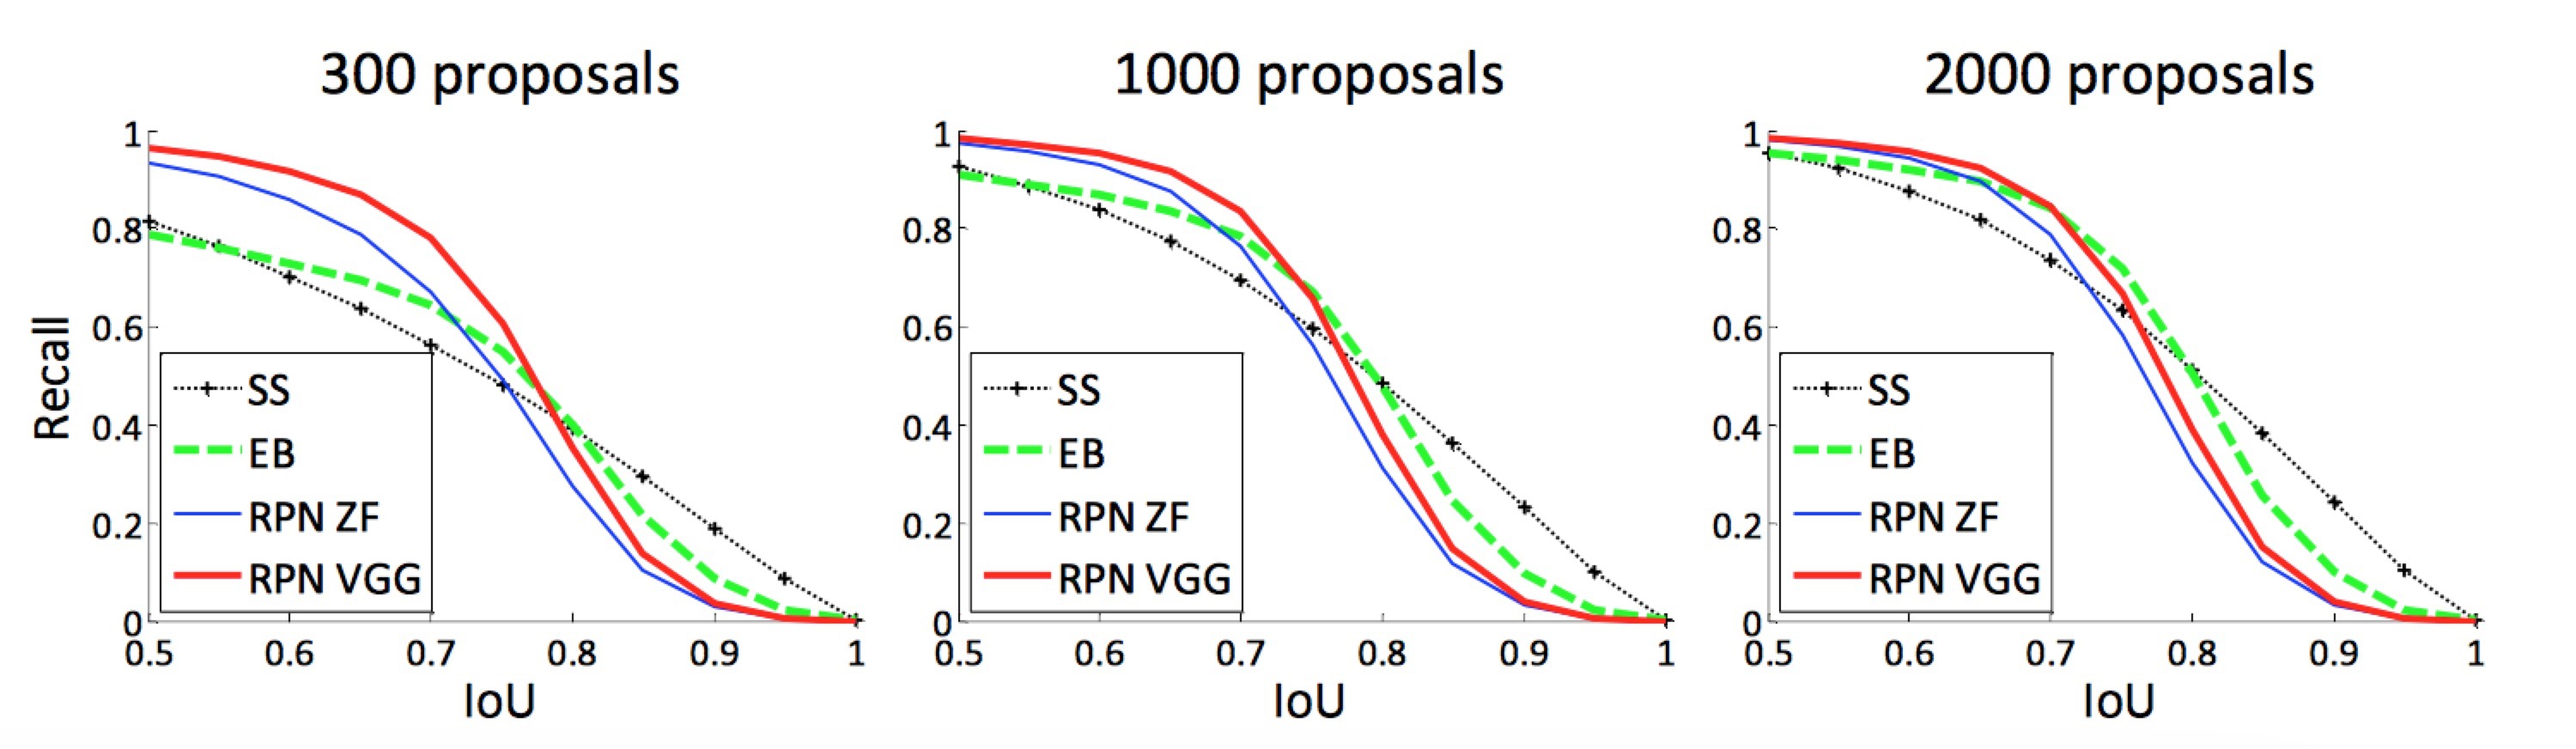
\includegraphics[width=\textwidth]{region-proposal}
	\caption{PASCAL VOC 2007测试集上的召回率 \textit{vs.} IoU阈值。SS:selective search,EB:edge box,RPN ZF:使用ZF Net \cite{zfnet} 模型,RPN VGG:使用VGG16 \cite{vgg} 模型。}
	\label{fig:region-proposal}
\end{figure}

RPN网络结构如图 \ref{fig:rpn} 所示。RPN使用的方法本质上就是滑动窗口。图 \ref{fig:rpn} 中的RPN使用了ZF Net模型,给定一张输入图像(假设分辨率为$600\times1000$),经过卷积操作得到最后一层的特征图(大约$40\times60$)。在这个特征图上使用$3\times3$的卷积核(滑动窗口)进行卷积,得到256张特征图,那么每个$3\times3$的区域经过卷积后都映射为一个256维的位置编码向量,后边再接两个并行的$1\times1$卷积层(\emph{cls} 层和\emph{reg} 层)分别用于分类和边框回归(跟Fast R-CNN类似,只不过这里只有目标和背景两个类别)。每个$3\times3$滑窗对应的位置编码向量同时预测3种尺度(128,256,512),3种长宽比(1:1,1:2,2:1)的region proposal,即图 \ref{fig:rpn} 中的$k=9$,这种映射的机制称为anchor。所以对于这个$40\times60$的特征图,总共有约20000($40\times60\times9$)个anchor,也就是预测20000个region proposal。RPN设计地比较巧妙,只需要在最后的卷积层上滑动一遍得到每个滑窗对应的位置编码向量,借助anchor机制就可以得到多尺度多长宽比的region proposal,加上后边接了边框回归,所以即便是这9种anchor之外的窗口也能得到一个跟目标比较接近的region proposal。

\begin{figure}[h]
	\centering
	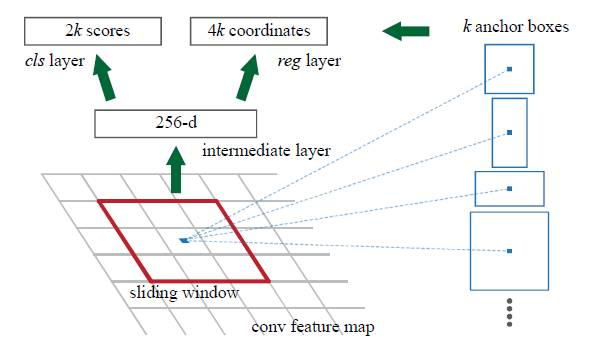
\includegraphics[width=0.8\textwidth]{rpn}
	\caption{RPN网络结构框图。图中$k$表示每个滑窗对应的anchor数目。}
	\label{fig:rpn}
\end{figure}

RPN看似巧妙的设计背后隐藏着一个假设:经过$3\times3$卷积后得到的位置编码向量能够包含足够多的信息来同时预测多个尺度的region proposal。然而实际情况是,每个位置编码向量在最后一层特征图(图 \ref{fig:rpn} 中的conv feature map)上的感受野(receptive field)是固定的,为$3\times3$,为后续分类和边框回归提供多尺度信息的能力有限。Cai等 \cite{mscnn} 通过实验证明,感受野固定和尺度变化之间的矛盾降低了RPN的召回率,尤其是对小目标的召回率。为了克服这一困难,本文采取的办法是获取最后一层特征图上每个位置在多个窗口大小下的位置编码,而不仅仅是$3\times3$的窗口大小。如图 \ref{fig:arpn} 所示,本文在每个位置分别获取$3\times3$,$5\times5$,$9\times9$,$17\times17$窗口大小的位置编码来感知多个尺度上的目标信息。在不同窗口大小上得到的位置编码用来对不同尺度的anchor进行分类和边框回归,例如图 \ref{fig:arpn} 中顶端的位置编码对尺度大小为64的anchors进行操作,而底部的位置编码对尺度大小为512的anchors进行操作。众所周知,卷积运算的计算量与卷积核的大小成正比,$17\times17$大小卷积核的计算量大约是$3\times3$大小卷积核的32倍。为了减少计算量,本文采用的卷积核为``带洞''的卷积核(atrous filter),即本文采取的卷积方式为atrous卷积。本文提出的方法被命名为Atrous Region Proposal Network(ARPN)。

\begin{figure}[h]
	\centering
	\includegraphics[width=\textwidth]{arpn}
	\caption{Atrous Region Proposal Network示意图。图中\texttt{conv5}表示最后一层特征图。}
	\label{fig:arpn}
\end{figure}

\subsubsection{Atrous卷积}
Atrous卷积最早被用于静态小波计算 \cite{atrous},近期在深度学习领域被用在语义分割(semantic segmentation)任务中 \cite{deeplab}。相比于标准卷积,atrous卷积能够在不增加卷积核参数和计算量的情况下,增大卷积核的感受野。以1-D信号为例,输入信号$x[i]$与一个长度为$K$的滤波器$f[k]$的atrous卷积输出$y[i]$定义为:
\begin{equation}\label{eqn:atrous}
	y[i] = \sum_{k=1}^{K} x[i+d*k]f[k]	
\end{equation}
其中$d$表示滤波器对输入信号的采样歩幅。在式 \ref{eqn:atrous} 的例子中,滤波器$f[k]$的等效长度变为$d\times(K-1)+1$。标准卷积是atrous卷积在$d=1$时的特殊情况。Atrous卷积可以看成在标准卷积核相邻的核值之间填充$d-1$个0。

\subsubsection{Atrous Region Proposal Network结构}
ARPN选用VGG16模型作为ARPN的基础网络。如图 \ref{fig:arpn} 所示,ARPN网络由四个并行的分支组成,在每个分支内有一个atrous卷积层进行位置编码,然后将这些位置编码传送给两个$1\times1$的卷积层分别进行对应anchors的分类和边框回归。这四个分支中atrous卷积核的真实大小均为$3\times3$,卷积核参数$d$从上至下依次为1,2,4,8,因而感受野的大小分别为$3\times3$,$5\times5$,$9\times9$,$17\times17$(如图 \ref{fig:arpn})。这四个分支的分类输出接下来在深度方向上叠加起来,得到所有尺度所有长宽比的anchors的分类结果,运用同样的方法,也可以得到这些anchors的边界框回归结果。本文采用4种尺度(64,128,256,512),3种长宽比(1:2,1:1,2:1)的anchors,所以图 \ref{fig:arpn} 中每个分支的\emph{cls}层输出维度为$2\times3=6$,\emph{reg}层输出维度为$4\times3=12$,最终将每个分支的输出层叠起来得到的\emph{cls}层输出维度为$6\times4=24$,\emph{reg}层输出维度为$12\times4=48$。

\subsubsection{ARPN训练}
在训练过程中,我们采用与RPN相同的策略将这些anchors标记为前景和背景。RPN采用的策略是计算每个anchor与所有ground-truth边界框的IoU,将满足下面任一条件的anchors标记为前景:
\begin{namelist}{}
	\item (1)与任意ground-truth边界框的IoU超过0.7。
	\item (2)对每个ground-truth边界框来讲,与它IoU最大的anchor。
\end{namelist}
并将满足以下条件的anchor标记为背景:与所有ground-truth边界框的IoU都不超过0.3。其余anchors不参与训练过程。训练过程中,一次minibatch随机采样256个正负样本,其中正负样本的比例设置为1:1,如果正样本不足128个,则使用所有正样本,剩下的样本从负样本中随机采样,反之亦然。ARPN训练使用的损失函数为:
\begin{equation}\label{eqn:loss}
L(\{p_i\},\{t_i\})=\frac{1}{N_{cls}}\sum_{i}L_{cls}(p_i,p_i^{*})+\lambda\frac{1}{N_{reg}}\sum_{i}p_i^{*}L_{reg}(t_i,t_i^{*})
\end{equation}
其中$i$是一个minibatch中anchor的索引,$p_i$是该anchor被预测为目标的概率,ground-truth $p_i^*$为1如果该anchor之前被标记为前景,$p_i^*$为0如果该anchor被标记为背景,$t_i$是预测的该anchor边框回归坐标,$t_i^*$是该anchor的ground-truth边框回归坐标,边框回归坐标的定义见下文。分类损失函数采用的是交叉熵,边框回归损失函数$L_{reg}=R(t_i-t_i^*)$,$R$函数采用的是Fast R-CNN中定义的Smooth L1 \cite{fast-rcnn},$p_i^*L_{reg}$意味着只对正样本统计回归误差。在ARPN中$N_{cls}$和$N_{reg}$均等于256。

边框回归坐标的定义如下:
\begin{equation}
t_x=(x-x_a)/w_a,\quad t_y=(y-y_a)/h_a,\quad t_w=\log(w/w_a), \quad t_h=\log(h/h_a)
\end{equation}
\begin{equation}
t_x^*=(x^*-x_a)/w_a,\quad t_y=(y^*-y_a)/h_a,\quad t_w^*=\log(w^*/w_a),\quad t_h^*=\log(h^*/h_a)
\end{equation}
其中$x,y,w,h$分别表示边框的中心以及宽高,$x,x_a,x^*$分别针对预测的边界框,anchor边界框和ground-truth边界框,$y,w,h$类似。式 \ref{eqn:loss} 中$t_i=(t_x, t_y, t_w, t_h)$,$t_i^*=(t_x^*,t_y^*,t_w^*,t_h^*)$。

本文使用在ImageNet上预训练好的VGG16模型对ARPN进行初始化,对于ARPN中新添加的层采用随机初始化。训练过程中,不同尺度anchor的误差被反向传播到对应的分支中去更新该分支中的卷机核。本文提出的ARPN方法通过不同感受野大小的卷积核从多个尺度上获取目标的位置编码,并在训练过程中给这些编码提供监督。这种方法通过下文的实验证明是有效,尤其是显著提高了小目标的召回率。

\subsubsection{实验结果}
本文将PASCAL VOC 2007测试集中的目标按照ground-truth边界框按的大小分为5组,并在这5组目标上分别对ARPN方法和RPN方法进行评估,评估指标选用的是J. Hosang等提出的Average Recall(AR)\cite{proposal}。当IoU阈值设置为0.5,0.6,0.7,0.8,0.9时各有一个region proposal对目标的召回率,AR就是这5个召回率的平均值。J. Hosang等通过大量实验证明,用AR来衡量region proposal质量的好坏是一个不错的选择,尤其是在目标检测领域。之后很多研究region proposal提取方法的学者都采用AR作为评价他们实验结果的指标。本文也选用AR指标来评估ARPN方法和RPN方法。VOC 2007数据集中包含5000张左右训练验证图像,5000张左右的测试图像。本文实验所用的训练集包含VOC 2007和VOC2012中的训练验证图像,共计约16.5k张图像,除了图像翻转没有做其他任何的数据增强。

本文选用Faster R-CNN作者释放出来的代码\footnote{\url{https://github.com/rbgirshick/py-faster-rcnn}},并使用默认的训练参数来训练一个用于提取region proposal的RPN网络。为了进行公平的比较,本文使用同样的参数来训练ARPN网络,它的实验结果以及与RPN的对比如表 \ref{tab:average_recall} 所示,表中对5组不同大小的目标分别进行了统计, ``small''表示目标面积位于区间$[0, 32^{2})$, ``medium''对应$[32^2, 96^2)$, ``96-128''对应 $[96^2, 128^2)$, ``128-256''对应 $[128^2, 256^2)$, ``256-512''对应 $[256^2, 512^2)$, ``all'':对应$[0, 512^2)$。从表 \ref{tab:average_recall} 中可以看出,对各种大小的目标,ARPN的表现都要胜出RPN,尤其是对小目标(Average Recall 提升了6.7\%)。而且提取300个region proposal的ARPN与提取2000个region proposal的RPN旗鼓相当。以上实验结果都表明本文提出的ARPN是一个比RPN更加优秀的region proposal提取算法,尤其是在本文要解决的周视监控场景下(会存在很多小目标)。
\begin{table}[h]
	\caption{ARPN和RPN在VOC 2007测试集上的Average Recall (\%). 本文根据ground-truth边界框的面积将目标分为5组 。对比中胜出的数字用黑色粗体表示。} %\R{Table updated.}}
	\centering
	\begin{tabular} {cc*{5}{c}c}
		\toprule
		method & \# proposals & small   & medium   & 96-128  & 128-256 & 256-512 & all\\
		\midrule
		\!\!\!\! RPN \!\!\!\!   & 2000 \!\!\!\! & 26.9 \!\!\!\! & 55.4 \!\!\!\! & 60.1 \!\!\!\! & 63.1 \!\!\!\! & 66.3 & 59.4 \!\!\!\! \\
		\!\!\!\! ARPN \!\!\!\!  & 2000 \!\!\!\! & \textbf{33.8} \!\!\!\! & \textbf{56.8} \!\!\!\! & \textbf{63.7} \!\!\!\! & \textbf{65.8} \!\!\!\! & \textbf{66.8} & \textbf{61.5} \!\!\!\! \\
	    \hline\hline
		\!\!\!\! RPN \!\!\!\!   & 300 \!\!\!\! & 25.3 \!\!\!\! & 50.6 \!\!\!\! & 53.4 \!\!\!\! & 61.2 \!\!\!\! & 66.2 & 56.4 \!\!\!\! \\
		\!\!\!\! ARPN \!\!\!\!  & 300 \!\!\!\! & \textbf{30.4} \!\!\!\! & \textbf{51.8} \!\!\!\! & \textbf{59.8} \!\!\!\! & \textbf{65.1} \!\!\!\! & \textbf{66.8} & \textbf{59.1} \!\!\!\! \\
		\bottomrule
	\end{tabular}%
	\label{tab:average_recall}%
\end{table}%

\subsection{Dense Fast R-CNN}
为了在目标检测场景下提高现有CNN网络对小目标的分类能力,本文提出了Dense Fast R-CNN。首先来分析Fast R-CNN为什么对小目标的分类能力不如尺度较大的目标。

深度卷积神经网络(DCNNs)最早被设计用来对图片进行分类,DCNN中周期性的降采样对图像分类任务是必要的,但是降采样导致的特征图分辨率降低对目标检测来讲是不利的,因为region proposal在特征图上对应的区域可能因为太小而不能为目标分类提供足够的信息,尤其是对小尺度region proposal。R-CNN通过将每个region proposal缩放到$227\times227$的大小解决了这个问题,但是需要对每个region proposal执行一遍DCNN的前向计算。Fast R-CNN加速了R-CNN的训练和测试过程,却没有解决特征图分辨率降低的问题。因为对于每个输入的region proposal,Fast R-CNN直接对它在最后一层卷积层(\texttt{conv5\_3})的投影区域进行池化操作得到用于后续类别分类和边界框回归的特征向量,然而\texttt{conv5\_3}在宽和高两个维度上的分辨率都只有输入图像的1/16,小尺度region proposal在\texttt{conv5\_3}上的投影区域的特征图不能包含足够的信息用于分类以及边界框回归。

为了提高对小目标的检测精度,最直接的方法就是多尺度输入(multi-scale input)的方案,但显著增加了内存和计算资源的消耗,限制了类似ResNet \cite{resnet} 这样深层神经网络的应用。Yang等 \cite{sdp} 提出了scale dependent pooling(SDP)池化机制,对小尺度的region proposal在浅层卷积特征图(分辨率高)进行池化,对尺度较大的region proposal在较深层卷积特征图(分辨率低)进行池化,并针对不同尺度的特征图训练不同的分类器。SDP能在一定程度上增强对小尺度目标的检测能力,但是相较于Fast R-CNN,它的参数数目显著增加,大量消耗内存,限制了该方法的应用范围。另外一种解决思路就是采用语义分割(semantic segmentation)领域中的方法来提高\texttt{conv5\_3}特征图的分辨率,备选的方案有SegNet \cite{segnet},Atrous Convolution Net \cite{deeplab},Deconvolution Net \cite{fcn} 等。带skip connection的反卷积网络(Deconvolution Net)需要归一化(normalize)不同层之间的激活值(activation),比较难训练;SegNet需要在原卷积网络的基础上额外增加Upsample层和卷积层,增大了网络的参数规模,而且新增加的层一般采用随机初始化;Atrous卷积可以fine-tune预先训练好的的网络,并且不会增加网络参数。本文采用atrous卷积(也称为dilated卷积)的方式来提高被池化卷积层(最后一层卷积层)的分辨率,进而提高对小尺度目标的检测精度。本文所提出的方法称作Dense Fast R-CNN。

\subsubsection{Dense Fast R-CNN网络结构}
如图 \ref{fig:dfrcn} 所示,Dense Fast R-CNN的网络结构依然可以分为卷积网络和RoI网络两部分,其中RoI网络的结构以及初始化方式均与Fast R-CNN保持一致,卷积网络由卷积层、MAX池化层以及atrous卷积层组成。Dense Fast R-CNN的卷积网络可以由FRCN的卷积网络进行如下变换得到:
\begin{namelist}{}
	\item (1)设置\texttt{pool4}(\texttt{conv4}后的MAX池化层)的池化歩幅为1,池化窗口的大小设置为$3\times3$,边界填充宽度设置为1(在Fast R-CNN中这些值分别为2,$2\times2$,0)。如图 \ref{fig:dilated} 所示,\texttt{pool4}的输出上采样了1倍。
	\item (2)\texttt{conv5}中包含的3个卷积层均使用atrous卷积,并设置每个卷积层的采样歩幅dilation=2,dilation表示式 \ref{eqn:atrous} 中的$d$,其余参数保持不变。由于\texttt{conv5}中的参数数目保持不变,依然可以使用VGG16模型进行Dense Fast R-CNN的初始化。如图 \ref{fig:dilated} 所示,初始化完成后,对比Dense Fast R-CNN和Fast R-CNN卷积网络的输出特征图(\texttt{conv5\_3})可以发现Dense Fast R-CNN输出的特征图分辨率更高,而且和Fast R-CNN的特征图具有相同的语义,验证了用预训练好的VGG16模型进行初始化的合理性。
\end{namelist}

\begin{figure}[t]
	\centering
	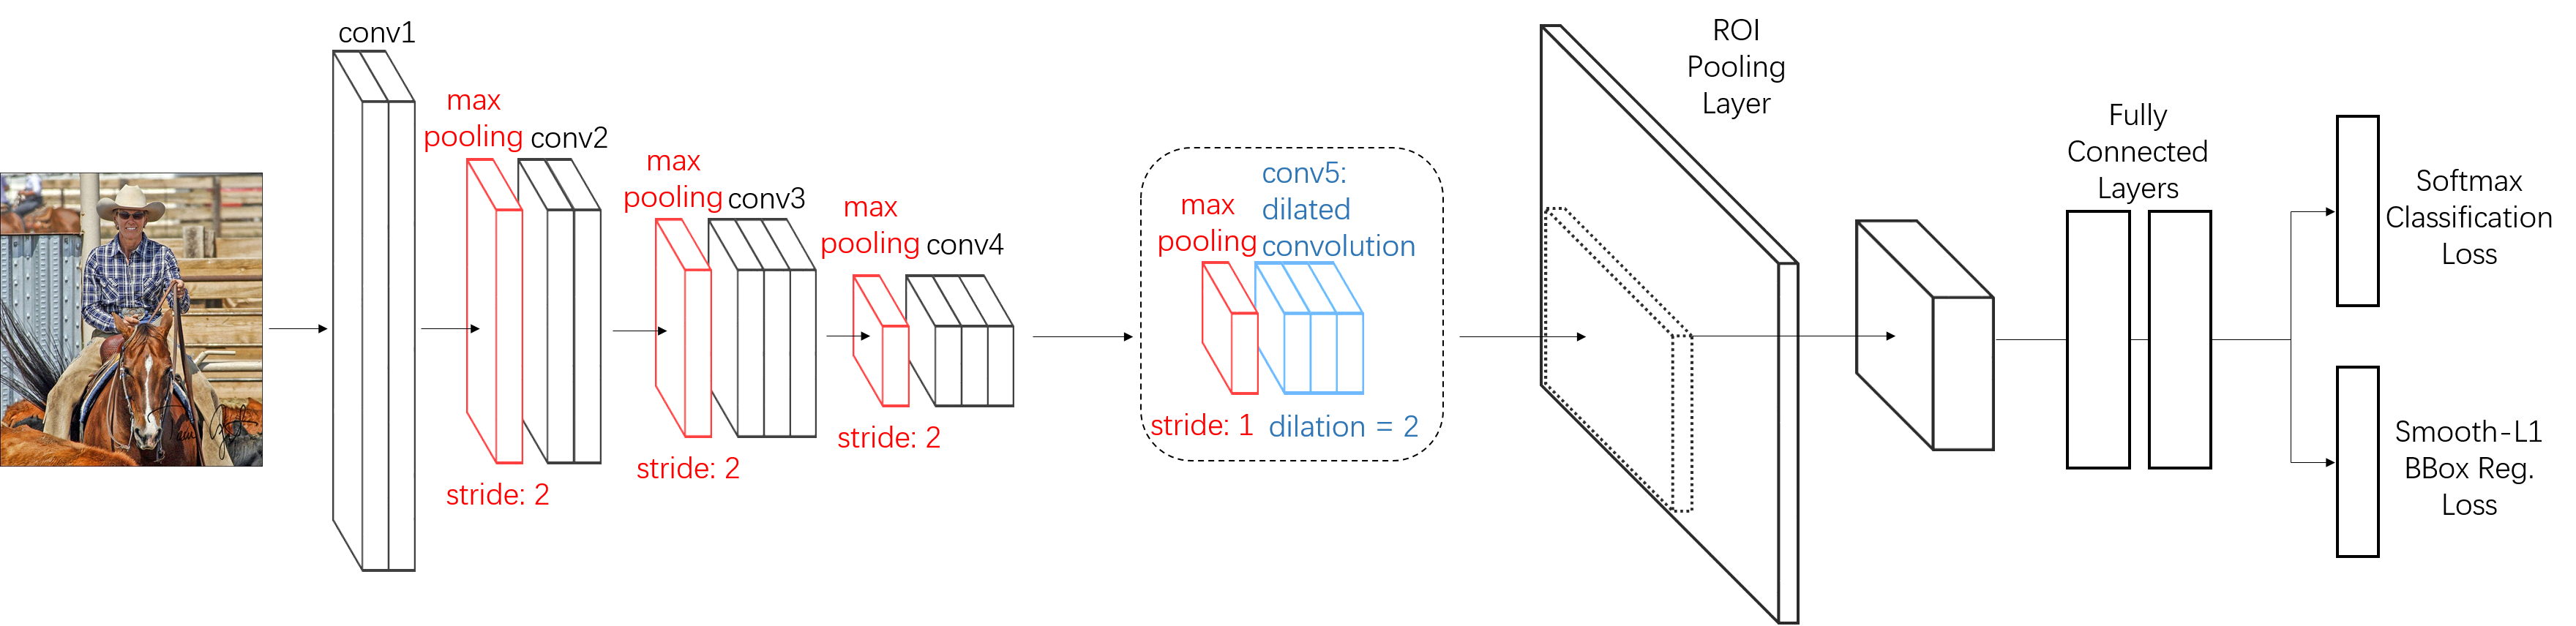
\includegraphics[width=\textwidth]{dfrcn}
	\caption{Dense Fast R-CNN目标检测流程图}
	\label{fig:dfrcn}
\end{figure}

\begin{figure}[h]
	\centering
	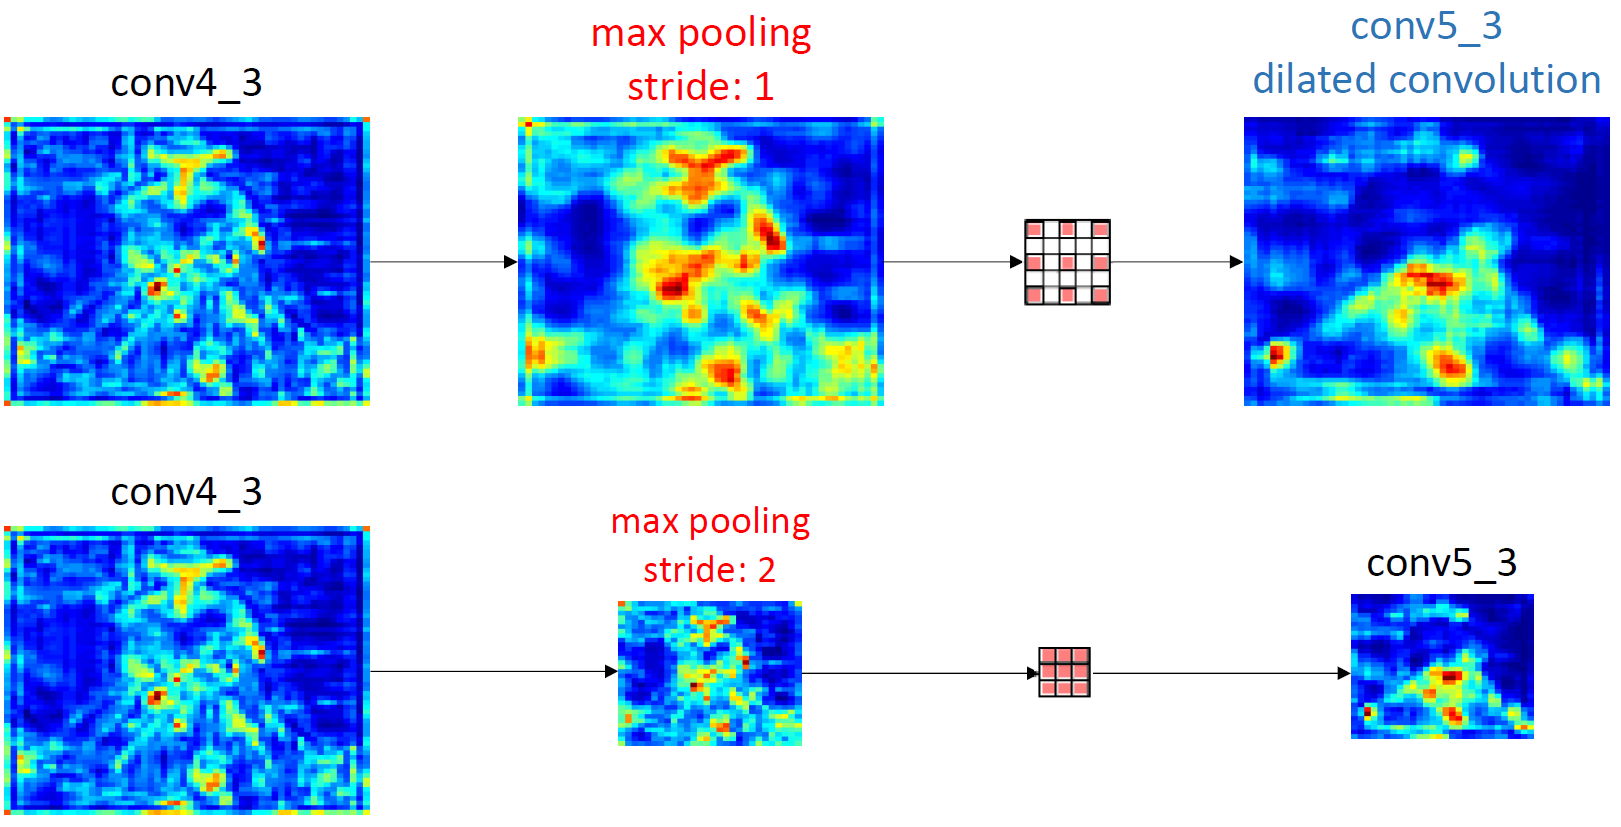
\includegraphics[width=0.8\textwidth]{dilated}
	\caption{将dilated(atrous)卷积引入Fast R-CNN前后,\texttt{conv5\_3}特征图分辨变化示意图。第一行:引入dialted卷积之后,第二行:原始Fast R-CNN特征图。}
	\label{fig:dilated}
\end{figure}

\subsubsection{实验结果}
与Dense Fast R-CNN相同,我们同样使用在ImageNet上预训练好的VGG16模型进行网络的初始化。训练数据集由PASCAL VOC2007的训练验证集以及VOC2012的训练验证集组成,共计约16.5k张图片。在本次实验中,Fast R-CNN和Dense Fast R-CNN使用的region proposal提取算法均为selective search \cite{selective-search}。 为了得到公平的比较结果,本文依然选用与Dense Fast R-CNN相同的SGD方式进行训练,同时保持训练参数一致。其中,我们设置初始学习率为0.001,每经过30k次迭代学习率减小到1/10,共迭代80k次。Dense Fast R-CNN在PASCAL VOC 2007上的评估结果及其与Fast R-CNN的对比如表 \ref{tab:dfrcn} 所示。本文提出的Dense Fast R-CNN方法提高了大部分类的检测精度,总体的检测精度为71.7\%,比Fast RCNN的70.0\%提高了1.7\%。同时Dense Fast R-CNN在包含小目标比较多的类别上,如bottle,plant,chair \cite{sdp} 分别提高了5.6\%,2.5\%,4.4\%,证明了Dense Fast R-CNN通过增加被池化特征图分辨率的方式提高了对小目标的分类能力。

\subsection{Atrous Faster R-CNN目标检测算法}
为了得到一个统一的目标检测框架,笔者将前文提出的Atrous Region Proposal Network,Dense Fast R-CNN结合起来,提出了Atrous Faster R-CNN目标检测算法。结合的方式与Faster R-CNN中RPN与Fast R-CNN结合的方式相同:RPN与Fast R-CNN共享卷积层的计算,然后RPN在最一层卷积层(\texttt{conv5\_3})输出的特征图上滑动得到约20000个候选窗口(具体数目与输入图像的分辨率有关),将这些候选按照置信度排序取前300个作为region proposal,有了region proposal和\texttt{conv5\_3}的特征图就可以用Fast R-CNN的方法进行目标检测了。注意在Atrous Faster R-CNN中由于\texttt{conv5\_3}的特征图上采样了一倍,为了节约计算量,笔者将ARPN在\texttt{conv5\_3}特征图上滑动的歩幅设置为2。

与前文相同,这里依然使用PASCAL VOC 2007和VOC2012训练验证集的组合作为训练样本集。训练后的模型在PASCAL VOC2007测试集上的评估结果如表 \ref{tab:dfrcn} 所示。Atrous Faster R-CNN的总体检测精度为76.9\%,比Faster R-CNN高出了3.7\%,在包含小目标比较多的种类,例如bottle,plant,chair上分别提高了11.4\%,13.9\%,8.8\%。

为了进一步对比目标大小对Faster R-CNN与Atrous Faster R-CNN检测精度的影响,本文提出了``average normalized area''的概念。图像中一个边界框的``normalized area''定义为该边界框的面积与图像的面积之比。测试数据集中一个目标类别的``average normalized area''定义为该测试集中所有类别标签为指定类别的ground-truth边界框的``normalized area''的平均值。``Average normalized area''能够反映一个目标类别的平均大小。如图 \ref{fig:rank} 所示,Atrous Faster R-CNN(ARPN+DFRCN)对小目标的检测精度提升更加明显,更加适用于周视监控的场景。本文提出的Atrous Faster R-CNN目标检测算法在Nvidia Titan X上的运行时间为230ms左右。
\begin{figure}[h]
	\centering
	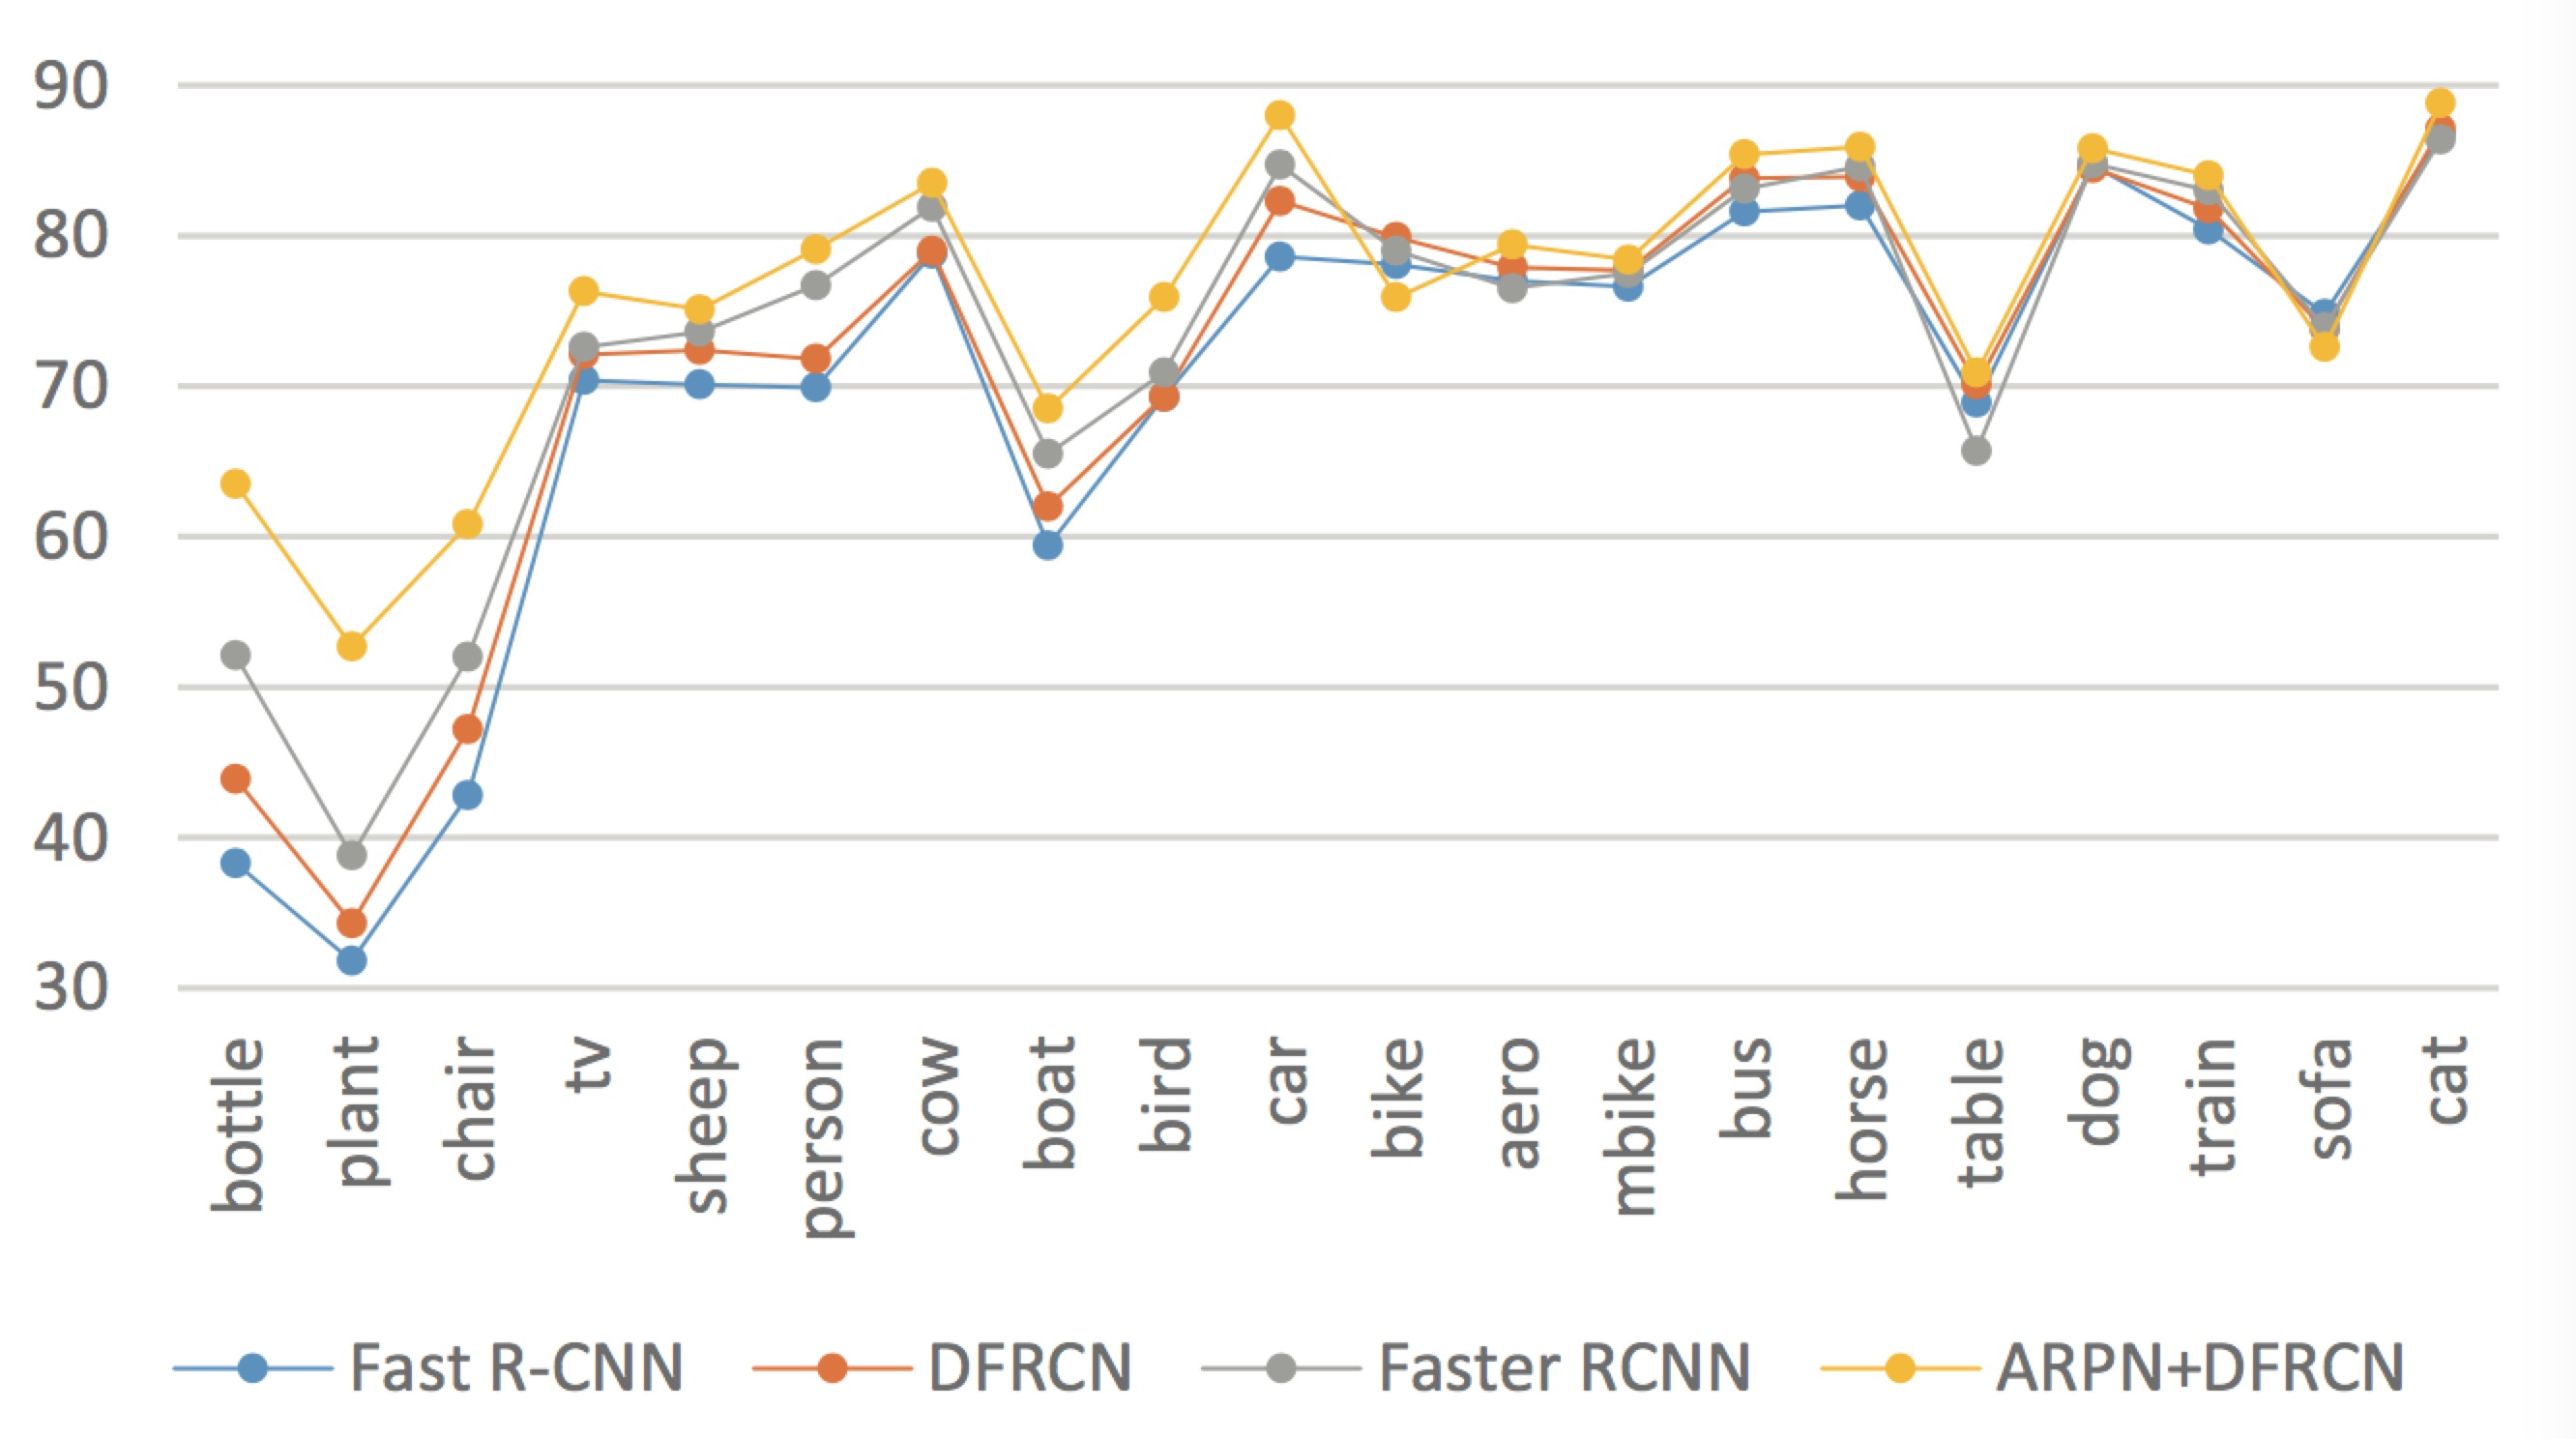
\includegraphics[width=\textwidth]{result}
	\caption{PASCAL VOC 2007测试集上的检测精度。目标类别按照``average normalized area''从小到大依次排列。}
	\label{fig:rank}
\end{figure}

\begin{sidewaystable}[h]
	\caption{VOC 2007测试集上的检测精度mAP(\%),图中显示4种犯法的检测结果,两种基准算法Fast R-CNCN and Faster R-CNN以及本文提出的算法Dense Fast R-CNN和Atrous Faster R-CNN(ARPN + DFRCN)。对比中胜出的数字用黑色粗体表示。}
	\centering
	\tiny
	\begin{tabular}{l|*{20}{c}|c}
		\hline
		method & aero & bike & bird & boat & bottle & bus & car & cat & chair & cow & table & dog & horse & mbike & persn & plant & sheep & sofa & train & tv & mAP\\
		\hline
		FRCN & 77.0 & 78.1 & 69.3 & 59.4 & 38.3 & 81.6 & 78.6 & 86.7 & 42.8 & 78.8 & 68.9 & \textbf{84.7} & 82.0 & 76.6 & 69.9 & 31.8 & 70.1 & \textbf{74.8} & 80.4 & 70.4 & 70.0 \\
		%\hline
		DFRCN & \textbf{77.9} & \textbf{79.9} & 69.3 & \textbf{62.0} & \textbf{43.9} & \textbf{83.8} & \textbf{82.3} & \textbf{87.1} & \textbf{47.2} & \textbf{79.0} & \textbf{70.1} & 84.5 & \textbf{83.9} & \textbf{77.7} & \textbf{71.8} & \textbf{34.3} & \textbf{72.4} & 73.8 & \textbf{81.8} & \textbf{72.1} & \textbf{71.7} \\
		\hline
		\hline
		Faster R-CNN & 76.5 & 79.0 & 70.9 & 65.5 & 52.1 & 83.1 & 84.7 & 86.4 & 52.0 & 81.9 & 65.7 & 84.8 & 84.6 & 77.5 & 76.7 & 38.8 & 73.6 & \textbf{73.9} & 83.0 & 72.6 & 73.2 \\
		ARPN + DFRCN & \textbf{79.4} & \textbf{84.1} & \textbf{75.9} & \textbf{68.5} & \textbf{63.5} & \textbf{85.4} & \textbf{88.0} & \textbf{88.8} & \textbf{60.8} & \textbf{83.5} & \textbf{70.9} & \textbf{85.8} & \textbf{85.9} & \textbf{78.4} & \textbf{79.1} & \textbf{52.7} & \textbf{75.1} & 72.6 & \textbf{84.0} & \textbf{76.3} & \textbf{76.9} \\
		\hline
	\end{tabular}
	\label{tab:dfrcn}
\end{sidewaystable}